\documentclass[aps,prl,twocolumn,
	groupedaddress,superscriptaddress,
	amsfonts,amssymb,amsmath,floatfix,
	citeautoscript]{revtex4-1}

\usepackage{graphicx}
\usepackage[centering,hmargin=20mm,tmargin=30mm,bmargin=25mm]{geometry}
\usepackage{multirow}
\usepackage{newtxtext}
\usepackage[cmintegrals]{newtxmath}

%----- References -----
\usepackage{xcolor}
\usepackage{hyperref}
\hypersetup{colorlinks,
	linkcolor={blue!75!black!80!yellow},
	citecolor={blue!75!black!80!yellow},
	urlcolor={blue!75!black!80!yellow}
}

%----- Captions in sans font -----
\makeatletter
\renewcommand\@make@capt@title[2]{%
	\@ifx@empty\float@link{\@firstofone}{\expandafter\href\expandafter{\float@link}}%
	\sffamily{\textbf{#1}}\@caption@fignum@sep#2
}%
\renewcommand\figurename{Fig.}
\makeatother

\thickmuskip=5mu plus 2mu minus 1mu  %binary relations (default, 5mu plus 5mu)
\medmuskip=4mu plus 2mu minus 2mu    %binary operations (default, 4mu plus 2mu minus 4mu)

\frenchspacing %Ensure that revTeX does not do "double spaces" after punctuation

\renewcommand{\Im}{\operatorname{Im}}
\renewcommand{\Re}{\operatorname{Re}}
\newcommand{\sub}[1]{\ensuremath{_{\textrm{#1}}}} %Upright multi-character subscript
\newcommand{\super}[1]{\ensuremath{^{\textrm{#1}}}} %Upright multi-character superscript

\newcommand{\HarvardSEAS}{John A. Paulson School of Engineering and Applied Sciences, Harvard University, Cambridge, MA, USA}
\newcommand{\MITPhy}{Department of Physics, Massachusetts Institute of Technology, Cambridge, MA, USA}

\usepackage[normalem]{ulem}
\newcommand{\Jadd}[1]{\textcolor{blue}{#1}}
\newcommand{\Jrem}[1]{\textcolor{blue}{\sout{#1}}}


%\usepackage[usenames]{color}
%\newcommand{\edited}[1]{{\color{red} #1}}

\begin{document}

\title{Variational theory of non-relativistic quantum electrodynamics}

\author{Nicholas Rivera}\email{nrivera@seas.harvard.edu}\affiliation{\HarvardSEAS}\affiliation{\MITPhy}
\author{Johannes Flick}\email{flick@seas.harvard.edu}\affiliation{\HarvardSEAS}
\author{Prineha Narang}\email{prineha@seas.harvard.edu}\affiliation{\HarvardSEAS}


\date{\today}

\begin{abstract}
The ability to achieve ultra-strong coupling between light and matter promises to bring about new means to control  material properties, new concepts for manipulating light at the atomic scale, and new insights into quantum electrodynamics (QED). Thus, there is a need to develop quantitative theories of QED phenomena in complex electronic and photonic systems. In this Letter, we develop a variational theory of general non-relativistic QED systems of coupled light and matter. Essential to our ansatz is the notion of an effective photonic vacuum whose modes are different than the modes in the absence of light-matter coupling. This variational formulation leads to a set of general equations that can describe the ground state of multi-electron systems coupled to many photonic modes in real space. As a first step towards a new  \textit{ab initio} approach to ground and excited state energies in QED, we apply our ansatz to describe a multi-level emitter coupled to many optical modes, a system with no analytical solution. We find a compact semi-analytical formula which describes ground and excited state energies to less than 1\% error in all regimes of coupling parameters allowed by sum rules. Additionally, our formulation provides a non-perturbative theory of Lamb shifts and Casimir-Polder forces, as well as suggesting new physical concepts such as the Casimir energy of a single atom in a cavity. Our method should thus give rise to highly accurate non-perturbative descriptions of many other phenomena in general QED systems. 
\end{abstract}

\maketitle

%\section{Introduction}
%\label{sec:Introduction}

Recent years have brought an explosion of progress in the study of light-matter interactions in the non-perturbative regime of quantum electrodynamics (QED)~\cite{flick7strong,ruggenthaler2017b,forn2018ultrastrong,baranov2018}. Ultra-strong, and even deep-strong coupling has been observed in systems involving superconducting qubits~\cite{blais2004,wallraff2004,forn2010observation,niemczyk2010circuit,yoshihara2017superconducting,forn2017ultrastrong}, large ensembles of molecules~\cite{hutchison2012,coles2014,coles2014b,shalabney2015coherent, thomas2016,ebbesen2016,stranius2018,thomas2018}, Landau level systems ~\cite{scalari2012ultrastrong,zhang2016collective},  quantum wells coupled to cavities ~\cite{todorov2010ultrastrong,geiser2012ultrastrong}, oscillators \cite{markovic2018demonstration}, and even in few-molecule systems ~\cite{benz2016,chikkaraddy2016}. Proposals for new platforms of ultra-strong coupling include emitters coupling to highly confined polaritons in metals and polar insulators \cite{rivera2016shrinking}, heavy ions coupled to optical media via the Cerenkov effect \cite{carmes2018non}, and many more. Proposed applications of ultra- and deep-strong coupling of light and matter are similarly broad, including simulation of many-body systems~\cite{forn2018ultrastrong}, altering chemical reactivity~\cite{hutchison2012, thomas2016,thomas2018, flick2017, herrera2016,feist2017,martinez2017} and electronic transport properties~\cite{orgiu2015} and realizing analogues of nonlinear optical processes with vacuum fluctuations~\cite{kockum2017deterministic}. Concomitantly with these developments are also theoretical developments in the study of QED systems \textit{ab initio}. Through `reduced quantity theories' such as quantum electrodynamical density functional theory (QEDFT)~\cite{tokatly2013,ruggenthaler2014,flick2015,dimitrov2017,flick2018,flick2018b}, one is now able to calculate observables in large molecules coupled to realistic optical cavities~\cite{flick2017c, flick2018b,flick2018}. 

In this Letter, we establish a variational framework to analyze complex light-matter systems from first principles. Although  \textit{ab initio} methods such as QEDFT are exact in principle and provide access to all observables, a number of practical difficulties arise related to: the lack of simple exchange-correlation functionals to describe the ground state energy, as well as other more involved observables, the difficulty of obtaining real-space information about the photons as they are affected by light-matter coupling, the difficulty of handling excited state energies, and the common use of the long-wavelength (dipole) approximation. A variational framework, as we show, flexibly allows a real-space description of the electrons and photons as they are modified by the coupling and also beyond the dipole approximation. Beyond these advantages, a variational framework also allows conceptual insights, as we shall show, into a simple non-perturbative theory of Lamb shifts, into a quasiparticle description of QED systems, and into the notion of Casimir forces in the limit of one atom. A variational framework also allows compact semi-analytical formulae to describe complex systems which may assist the development of functionals for use in QEDFT. 
 %In the nonperturbative regime of quantum electrodynamics, there are very few models which can be analytically solved. In particularly, the only exactly solvable models in all regimes of coupling parameters include the Rabi model~\cite{braak2011}, which describes the coupling of a two-level atom to a single mode, the Hopfield model \cite{hopfield1958theory}, which describes the coupling of a harmonic oscillator to any number of cavity modes, and Dicke models based on two-level systems and harmonic oscillators \cite{dicke1954coherence}. Any realistic system which deviates from these simpler models require numerical diagonalization approaches for an exact solution, which become unwieldy when the dimension of the electronic Hilbert space becomes large, as is the case when describing an electronic system in real space. It also becomes unwieldy when one needs to keep track of many cavity modes which can also be populated with many photons. Exciting new developments towards ab-initio studies of QED have proceeded by proposing reduced-quantity descriptions such as density-functional descriptions of the light-matter coupling \cite{ruggenthaler2014,pellegrini2015,flick2015,dimitrov2017,flick2018,flick2018b,schaefer2018}. With such density-functional descriptions, workers in this field have been able to compute ground-state and time-dependent properties of realistic molecules in optical cavities \cite{flick2017c}. 

Motivated by all of these potential advantages, we now develop an ansatz in which the ground state can be considered as a factorizable state of effective matter and effective photon quasiparticles, both in their respective vacuum states. This ansatz $-$ reminiscent to, but qualitatively distinct from, the Hartree-Fock ansatz~\cite{szabo1989} of electronic structure theory $-$ leads to coupled eigen-equations describing ground and excited states of the light-matter system. We apply our ansatz to describe ground and excited states in a multi-level emitter coupled to many photonic modes. We find that for light-matter couplings that respect sum rules, our method yields ground and excited state energies to a remarkable accuracy of up to 99\%, even in deeply non-perturbative coupling regimes.  In regimes where our results are accurate, we have found the effective quasiparticle description of the ground state of QED.  Our findings also furnish a non-perturbative theory of the position-dependent energy (Lamb) shifts of ground and excited states that give rise to Casimir-Polder forces. \textcolor{blue}{The variational method put forth developed in this manuscript is particularly suited for dealing with QED systems in the ultrastrong coupling regime, in which the rotating-wave approximation no longer holds, and subsequently methods based on the Jaynes-Cummings model such as dressed state approaches \cite{cohen1992} are no longer accurate.} Moreover, our approach is particularly suited to scalably dealing with systems with many emitter levels, as well as many cavity modes which may have large virtual photon occupation numbers.


%Our results service several aims. First, they suggest a novel variational approach for understanding ground states in ultra-strongly coupled light-matter systems. Second, they provide a general framework for understanding light-matter decoupling effects in the regime of strong light-matter interactions. Third, they prove a non-perturbative theory of Casimir-Polder forces \Jadd{(cite)}. Finally, they provide a rigorous concept of correlation energy in quantum electrodynamics in a way analogous to electronic structure theory. 

%The outline of this work is as follows: in section~\ref{sec:variational_ansatz}, we develop the variational ansatz for the ground state of the Hamiltonian of macroscopic quantum electrodynamics. In section~\ref{sec:multi-level}, we calculate the ground state energy according to this ansatz for the multi-level and multi-mode Rabi model and compare it to numerical diagonalization of the same problem. In Section~\ref{sec:extensions}, we propose a self-consistent extension of our ansatz. 

The QED Hamiltonian is given by $H = H_{\mathrm{mat}}+H_{\mathrm{em}}+H_{\mathrm{int}}$ where $H_{\mathrm{mat}}$ describes the matter in the absence of the quantized electromagnetic field, $H_{\mathrm{em}}$ describes the photons in the absence of the matter, and $H_{\mathrm{int}}$ describes the coupling between light and matter. The matter Hamiltonian takes the form:
\begin{align}
H_{\mathrm{el}} &= \int d^3x ~\psi^{\dagger}(\mathbf{x})\left(-\frac{\hbar^2\nabla^2}{2m} + v_{\mathrm{ext}}(\mathbf{x}) \right)\psi(\mathbf{x}) \nonumber \\ &+ \frac{1}{2}\int d^3x d^3x'~ \psi^{\dagger}(\mathbf{x})\psi^{\dagger}(\mathbf{x}')V(\mathbf{x}-\mathbf{x}')\psi(\mathbf{x}')\psi(\mathbf{x}),
\end{align}
where $v_{\mathrm{ext}}$ is the one-body external potential, $V(\mathbf{x}-\mathbf{x}')$ is the two-body interaction kernel, and $\psi$ is the second-quantized electron field. %\Jadd{(shouldn't x also be bold when it is an argument, since it a vector)}
\begin{figure}[t]
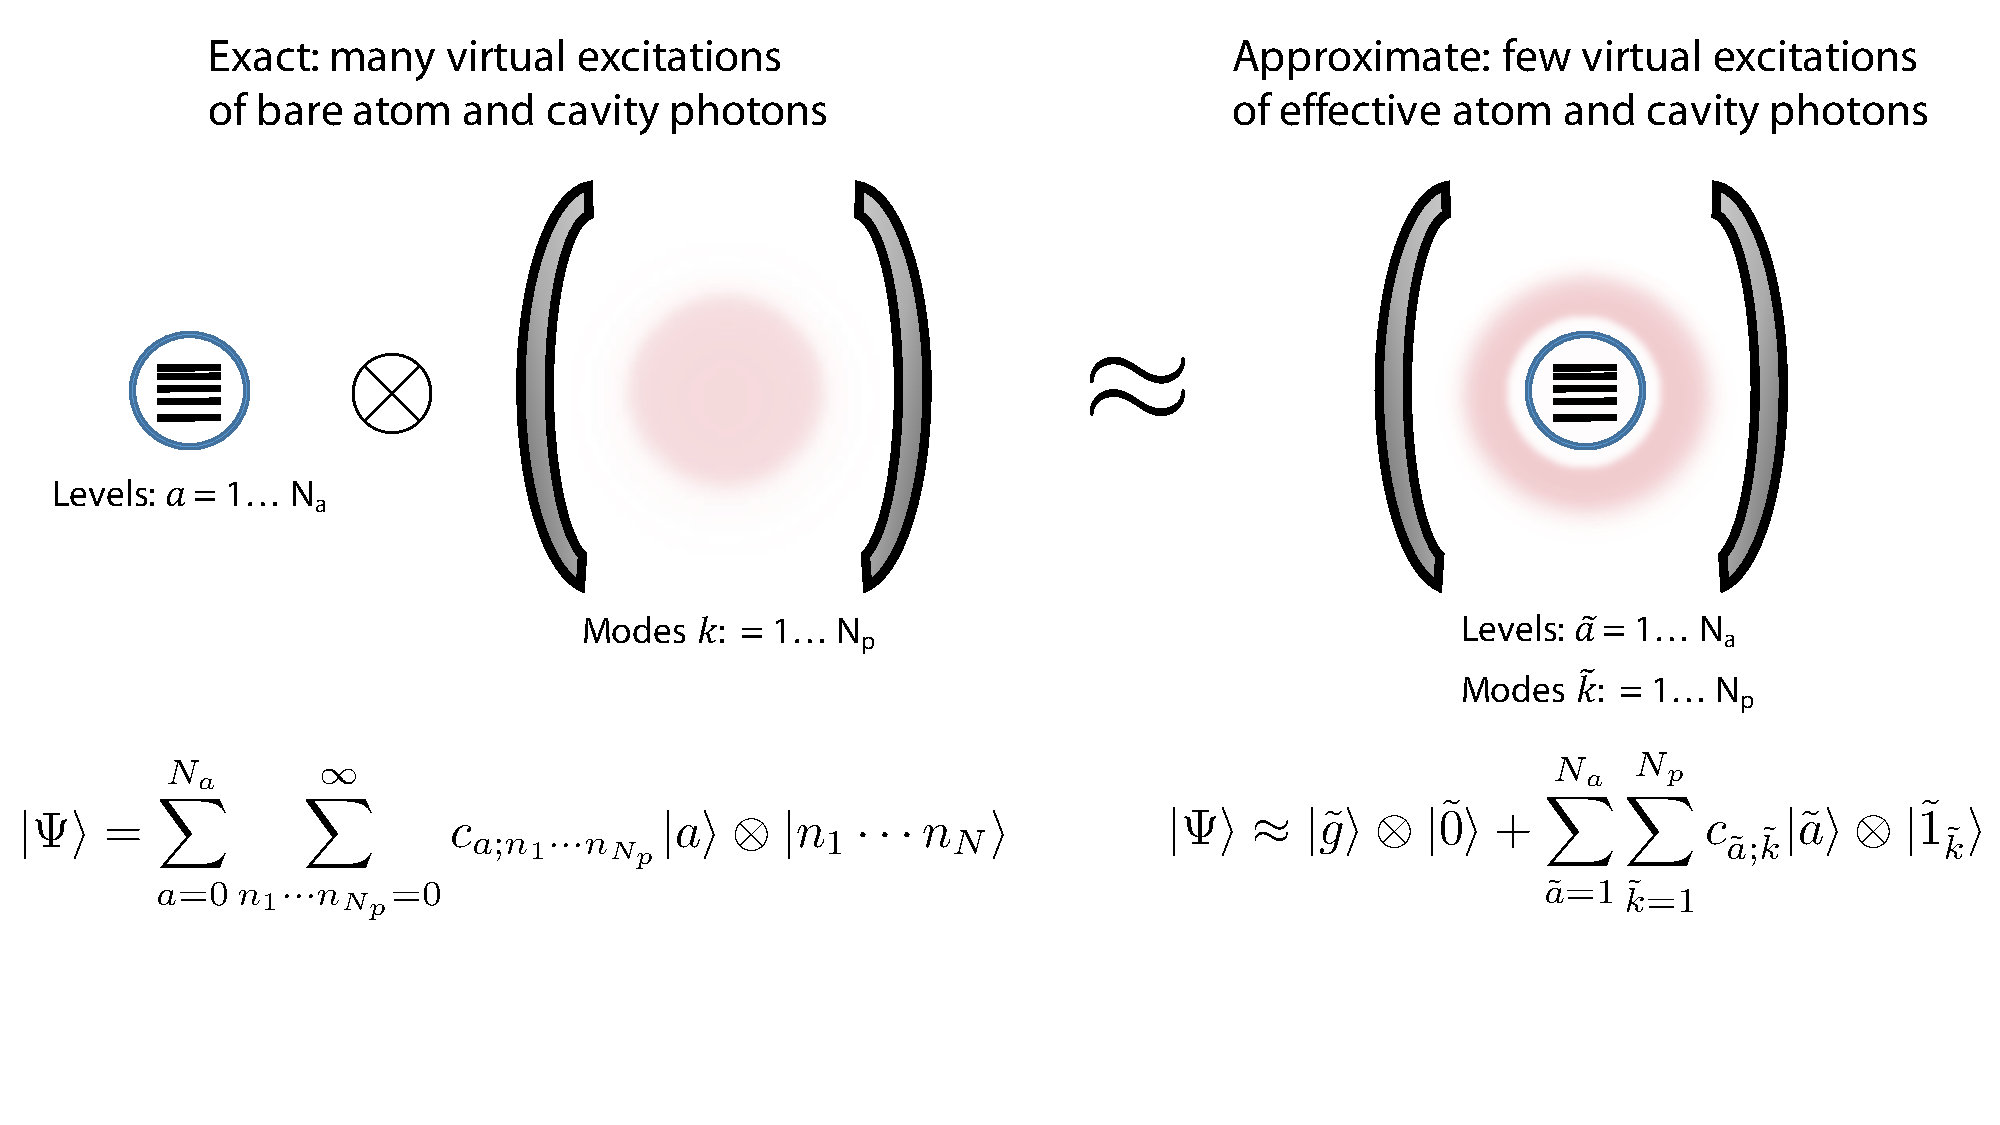
\includegraphics[width=8.5cm]{conceptfigure.pdf}
\caption{\textbf{Ground-state ansatz applied to matter in a cavity: effectively decoupled matter and photons.} (Left) Bare description of the coupled light-matter ground state in terms of many virtual excitations of the emitter state and the bare cavity photons. (Right) Quasiparticle description of the coupled system as a factorizable state of an effective emitter in its ground state and the vacuum of an effective photonic degree of freedom.}
\label{fig:ansatz}
\end{figure}
Parameterizing the electromagnetic field purely in terms of a vector potential: $\mathbf{E} = -\partial_t\mathbf{A}$ and $\mathbf{B} = \nabla\times\mathbf{A}$ renders the free electromagnetic Hamiltonian as
\begin{equation}
H_{\mathrm{em}} = \frac{\epsilon_0}{2}\int d^3x~ \epsilon (\partial_t \mathbf{A}(\mathbf{x}))^2 + \mathbf{A}(\mathbf{x})\cdot(\nabla\times\mu^{-1}\nabla\times\mathbf{A}(\mathbf{x})),
\end{equation}
where $\epsilon$ and $\mu$ represent a non-dispersive and positive dielectric and magnetic background that the matter and photon occupy. For cases we consider in this work, these will be taken to be unity.

The interaction Hamiltonian takes the form:
%\begin{align}
%H_{\mathrm{int}} = &\frac{-i\hbar e}{2m}\int d^3x ~\psi^{\dagger}(\mathbf{x})(\mathbf{A}\cdot\nabla +  \nabla \cdot \mathbf{A})\psi(\mathbf{x}) + \nonumber \\ &\frac{e^2}{2m}\int d^3x ~\psi^{\dagger}\psi\mathbf{A}^2(\mathbf{x}).
%\end{align}
\begin{align}
H_{\mathrm{int}} &= \frac{-i\hbar e}{2m}\int d^3x ~\psi^{\dagger}(\mathbf{x})(\mathbf{A}(\mathbf{x})\cdot\nabla +  \nabla \cdot \mathbf{A}(\mathbf{x}))\psi(\mathbf{x}) \nonumber \\ &+ \frac{e^2}{2m}\int d^3x ~\psi^{\dagger}(\mathbf{x})\psi(\mathbf{x})\mathbf{A}^2(\mathbf{x}).
\end{align}

The full Hamiltonian $H$, which depends on the fields $\psi$ and $\mathbf{A}$ can be parameterized in terms of an orthonormal set of electron single-particle wavefunctions (orbitals) $\{\psi_n\}$, and in terms of a set of photonic mode functions (orbitals) $\{\mathbf{F}_i\}$. The electron field operator takes the form $\psi(\mathbf{x}) = \sum_n \psi_n(\mathbf{x})c_n$.
The $c_n$ is an annihilation operator for an electron corresponding to state $n$. The electromagnetic field operator takes the form $\mathbf{A}(\mathbf{x}) = \sum_i\sqrt{\frac{\hbar}{2\epsilon_0\omega_i}} \left(\mathbf{F}_i(\mathbf{x})a_i+\mathbf{F}^*_i(\mathbf{x})a^{\dagger}_i\right)$, where the $a_i^{(\dagger)}$ annihilate (create) a photon in mode $i$. In the electromagnetic field operator, we parameterize not only by the mode functions but also by mode frequencies. The normalization chosen for the electron wavefunctions is $\int d^3x~ \psi_m^*\psi_n = \delta_{mn}$ while for the photon mode functions, it is $\int d^3x~\epsilon\mathbf{F}_i^*\cdot\mathbf{F}_j = \delta_{ij}$ \cite{joannopoulos2011photonic}.

Given an ansatz $|\Omega\rangle$ for the ground state of $H$, the variational theorem ensures that $\langle \Omega|H|\Omega\rangle$ is an upper bound for the ground state energy. Parameterizing $|\Omega\rangle$ to generate a family of ground states, and minimizing $\langle \Omega|H|\Omega\rangle$ with respect to the introduced parameters gives the best upper bound for the ground state energy within this family of ground states.  We choose as our ansatz
\begin{equation}
|\Omega\rangle = \left( \prod\limits_n c_n^{\dagger}|0_n\rangle\right) \otimes \left(\bigotimes_i|0_i\rangle\right).
\label{eq:ansatz}
\end{equation}
where, $\prod\limits_n c_n^{\dagger}|0_n\rangle$ represents a `filled Fermi sea' for effectively non-interacting electrons, and $\left(\bigotimes_i|0_i\rangle\right)$ represents a `photonic vacuum' for effectively non-interacting photons (see Fig. ~\ref{fig:ansatz}). Implicitly, this ansatz, once we take the expectation value $\langle \Omega|H|\Omega\rangle$, denotes a family of ansatzes labeled by all possibilities for the electron wavefunctions,  photon mode functions, and photon mode frequencies. Thus, we minimize the expectation value with respect to $\psi_n, \psi_n^*, \mathbf{F}_i, \mathbf{F}_i^*$, and $\omega_i$.  We enforce that the matter and photon remain normalized by constructing the Lagrange function:
\begin{align}
&\mathcal{L}[\{ \psi_n,\psi_n^* \},\{ \mathbf{F}_i,\mathbf{F}_i^*,\omega_i \}] = \langle \Omega |H|\Omega\rangle \\
&- \sum_n E_n\left(\int d^3x ~\psi_n^*\psi_n - 1 \right) - \sum_i \frac{\hbar\lambda_i}{2}\left(\int d^3x ~\epsilon\mathbf{F}_i^*\cdot\mathbf{F}_i - 1 \right),\nonumber
\end{align}
with the $E_n$ and $\frac{\hbar\lambda_i}{2}$ being the Lagrange multipliers that enforce the normalization conditions. Evaluating the expectation value of the Hamiltonian, and minimizing the Lagrange function  immediately yields:
\begin{align}
&\left(\frac{\mathbf{p}^2}{2m}+v_{\mathrm{ext}}(\mathbf{x}) \right)\psi_i(\mathbf{x}) + \nonumber \\ &\sum\limits_{j=1}^N \int d^3x' ~ V(\mathbf{x}-\mathbf{x}')\psi^*_j(\mathbf{x}')\psi_j(\mathbf{x}')\psi_i(\mathbf{x}) \nonumber \\ & - \sum\limits_{j=1}^N \int d^3x' ~ V(\mathbf{x}-\mathbf{x}')\psi^*_j(\mathbf{x}')\psi_j(\mathbf{x})\psi_i(\mathbf{x}')  \nonumber \\ &+ \frac{\hbar e^2}{4m\epsilon_0}\left(\sum_n \frac{1}{\omega_n}|\mathbf{F}_n|^2\right)\psi_i(\mathbf{x})   = E_i\psi_i(\mathbf{x}),
\label{eq:mhf-electron}
\end{align}
for the electron orbitals and energies. We see that in addition to the one-body and Hartree-Fock terms for the electrons, the effect of the QED coupling is to add a one-body ponderomotive potential. %We note that in the often used dipole approximation, the ponderomotive potential has no effect as it becomes independent of position.

For the photon orbitals and energies, the minimization yields:
\begin{equation}
\left( \nabla\times\nabla\times - \frac{\omega_i^2}{c^2}\left(1-\frac{\omega_p^2(\mathbf{x})}{\omega_i^2} \right)\right)\mathbf{F}_i = 0,
\label{eq:mhf-photon}
\end{equation}
where $\omega_p^2(\mathbf{x}) = \frac{e^2}{m\epsilon_0}\sum\limits_{n=1}^N |\psi_n(\mathbf{x})|^2$ is a position-dependent squared-plasma frequency which will push the photon orbitals out of the region where the emitter is located. Equations (\ref{eq:mhf-electron}) and (\ref{eq:mhf-photon}) are main results and can be used to describe ultra-strongly coupled systems in three dimensions, in an arbitrary photonic system, and with multi-electron matter. Excited states in this framework can be identified with matter and photon quasiparticle excitations.

Note that term in the interaction Hamiltonian linear in the vector potential (the "$A\cdot p$ term") makes no contribution to the expectation value of the ground state of the energy in this ansatz. At second order in the $A\cdot p$ term, virtual photon processes arise, such as Lamb shifts, whose emitter-position-dependence gives rise to van der Waals and Casimir-Polder forces  \cite{scheel2009macroscopic}.  Physically, this term will mix the factorizable ground state of Eq.~(\ref{eq:ansatz}) with states that simultaneously have virtual excitations of the matter and the electromagnetic field. The resulting state is non-factorizable and thus, the term in the $A\cdot p$ term leads to \textit{correlations} in the system, and contributes wholly at lowest order to the correlation energy of QED ground and excited states. We note that correlations can also be included in the energy shifts of excited emitter states, as well as states that already have photonic excitations \footnote{The behavior of the $A\cdot p$ and $A^2$-term is similar to the ${r}\cdot D$ and $r^2$ term in the length-gauge reported in recent work on the optimized effective potential~\cite{pellegrini2015,flick2017c} method for QEDFT including one-photon processes. }.
\begin{figure}[t]
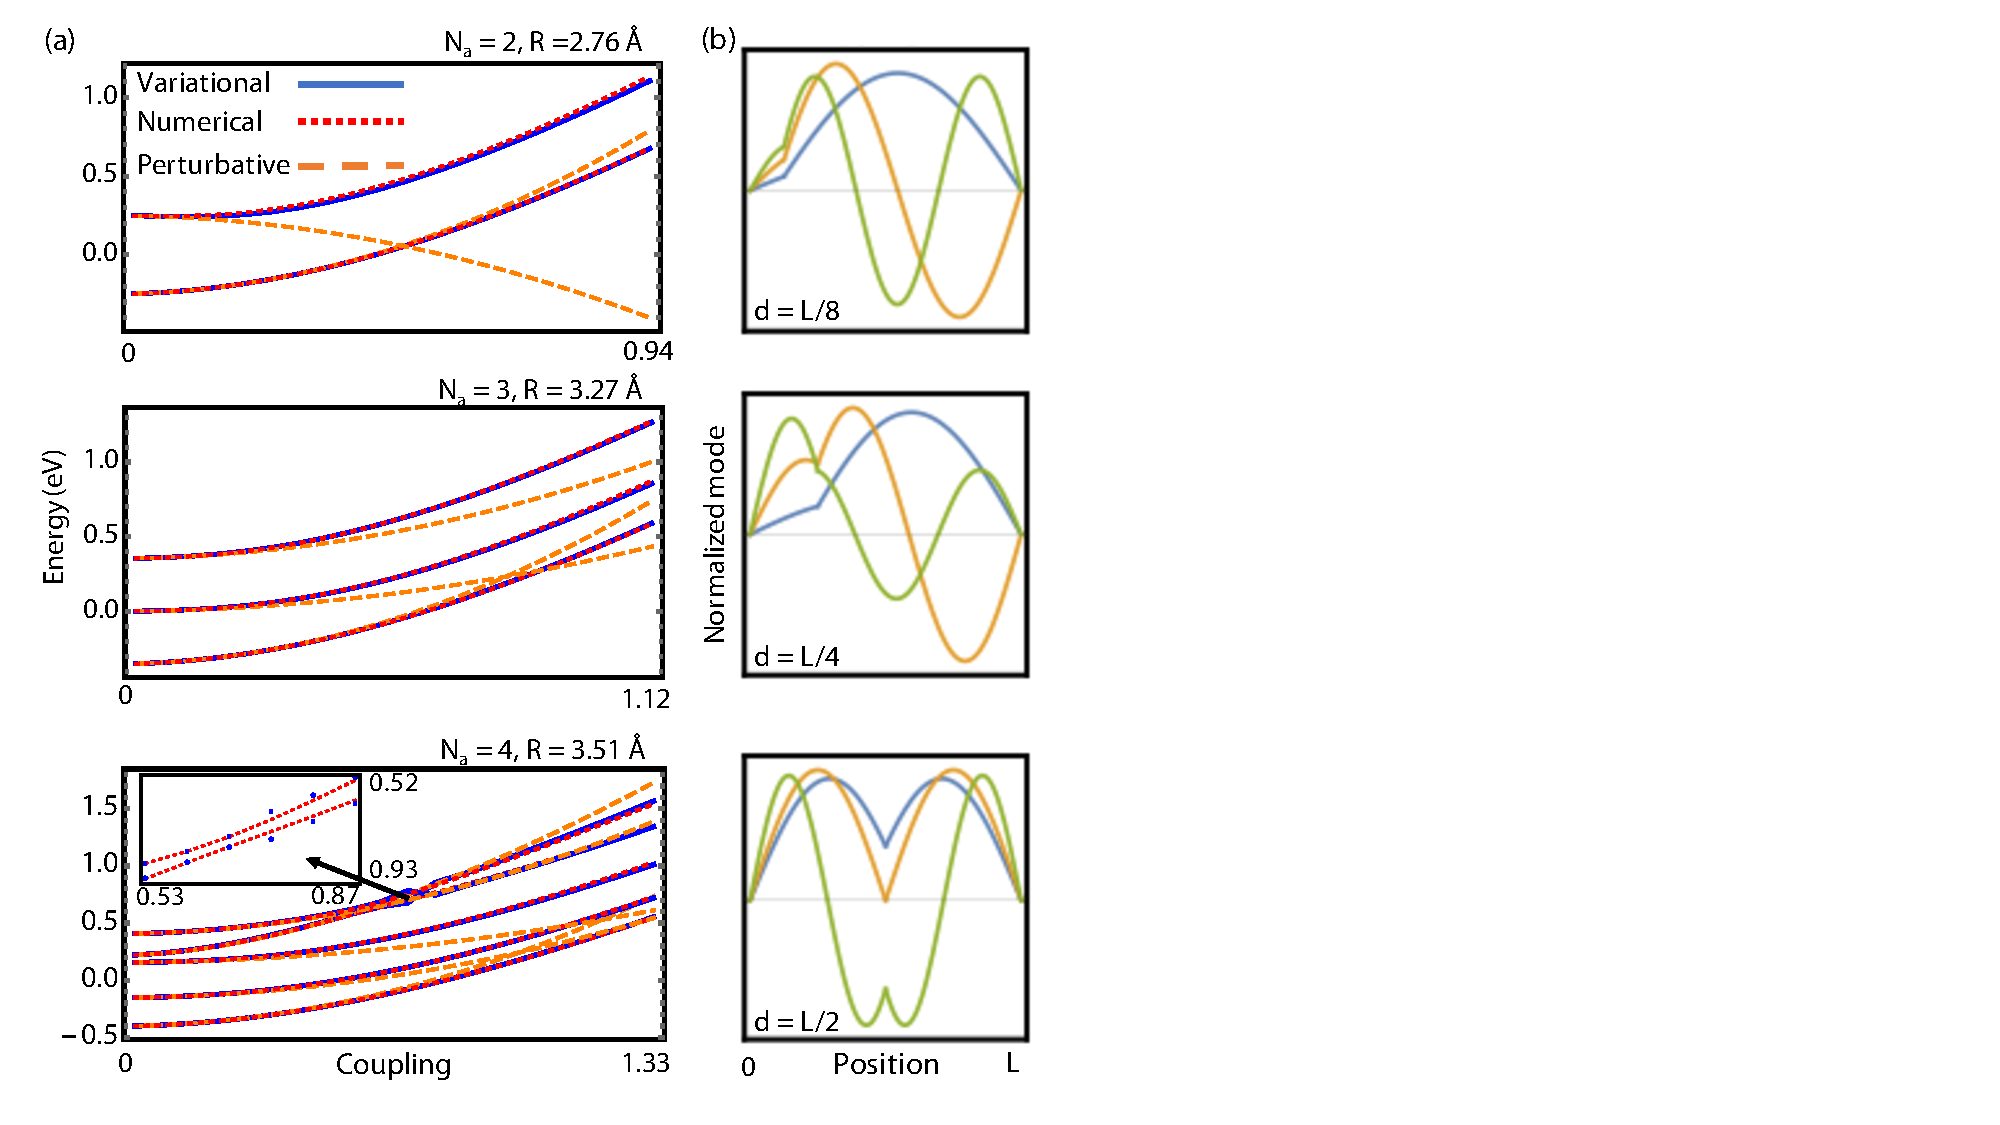
\includegraphics[width=8.5cm]{Figure2and3combined.pdf}
\caption{\textbf{Variational theory of ground and excited states in non-perturbative QED.} (a) Lowest few energy levels of a two (top), three (middle), and four (bottom) level system embedded in the middle of a one-dimensional cavity. The results of the variational method (blue) are compared to perturbation theory (orange), as well as numerical diagonalization (red) with the Fock space truncated to fifty cavity modes with no more than four photons. (Inset) The fourth and fifth energy levels show a weak anti-crossing behavior which is well-reproduced by the variational theory. Blue denotes variational while red denotes numerical. (b) Mechanism of overestimation of couplings and resonances in perturbation theory: modes derived from the variational theorem are suppressed in the vicinity of the emitter, which self-consistently decreases the field-emitter coupling.  }
\label{fig:results}
\end{figure}

We capture the effect of correlations perturbatively. For the ground state, we consider the second-order correction $\delta E$ to the ground state energy arising from the term in the Hamiltonian linear in the vector potential. That correction is given by 
\begin{equation}
\delta E = \frac{e^2\hbar^2}{8m^2\epsilon_0}\sum\limits_{i=1}^{\infty}\sum_{n=N_{\sigma}+1}^{\infty}\sum\limits_{m=1}^{N_{\sigma}} \frac{\Big| \int d^3x~\mathbf{F}_i^*\cdot\mathbf{j}_{nm}\Big|^2}{\omega_i(\omega_{mn} -\omega_i)},
\label{eq:e-shift}
\end{equation}
where $\mathbf{j}_{nm} = \psi^*_n\nabla\psi_m - (\nabla\psi^*_n)\psi_m$, $\omega_{mn} = \omega_m - \omega_n$, and$N_{\sigma}$ is the number of occupied orbitals, equal to the number of electrons.  In a method without self-consistency, the electron and photon orbitals and eigenvalues are those obtained from Eqs. (\ref{eq:mhf-electron}) and (\ref{eq:mhf-photon}), and then the electron energies and orbitals as well as the photon frequencies and orbitals, are plugged into Eq. (\ref{eq:e-shift}). By taking $m$ as an ansatz for an excited state, correlation corrections to excited states can also be found. \textcolor{blue}{In the Supplementary Information, we derive a set of equations for the matter orbitals and photonic mode functions which self-consistently takes into account the correlation energy associated with Eq. ~\ref{eq:e-shift}. These equations take into account the spatially varying wavefunctions to the spatially varying mode functions, just like Eqs. \ref{eq:mhf-electron} and \ref{eq:mhf-photon}, and therefore do not assume the dipole approximation.}
%\begin{figure}[t]
%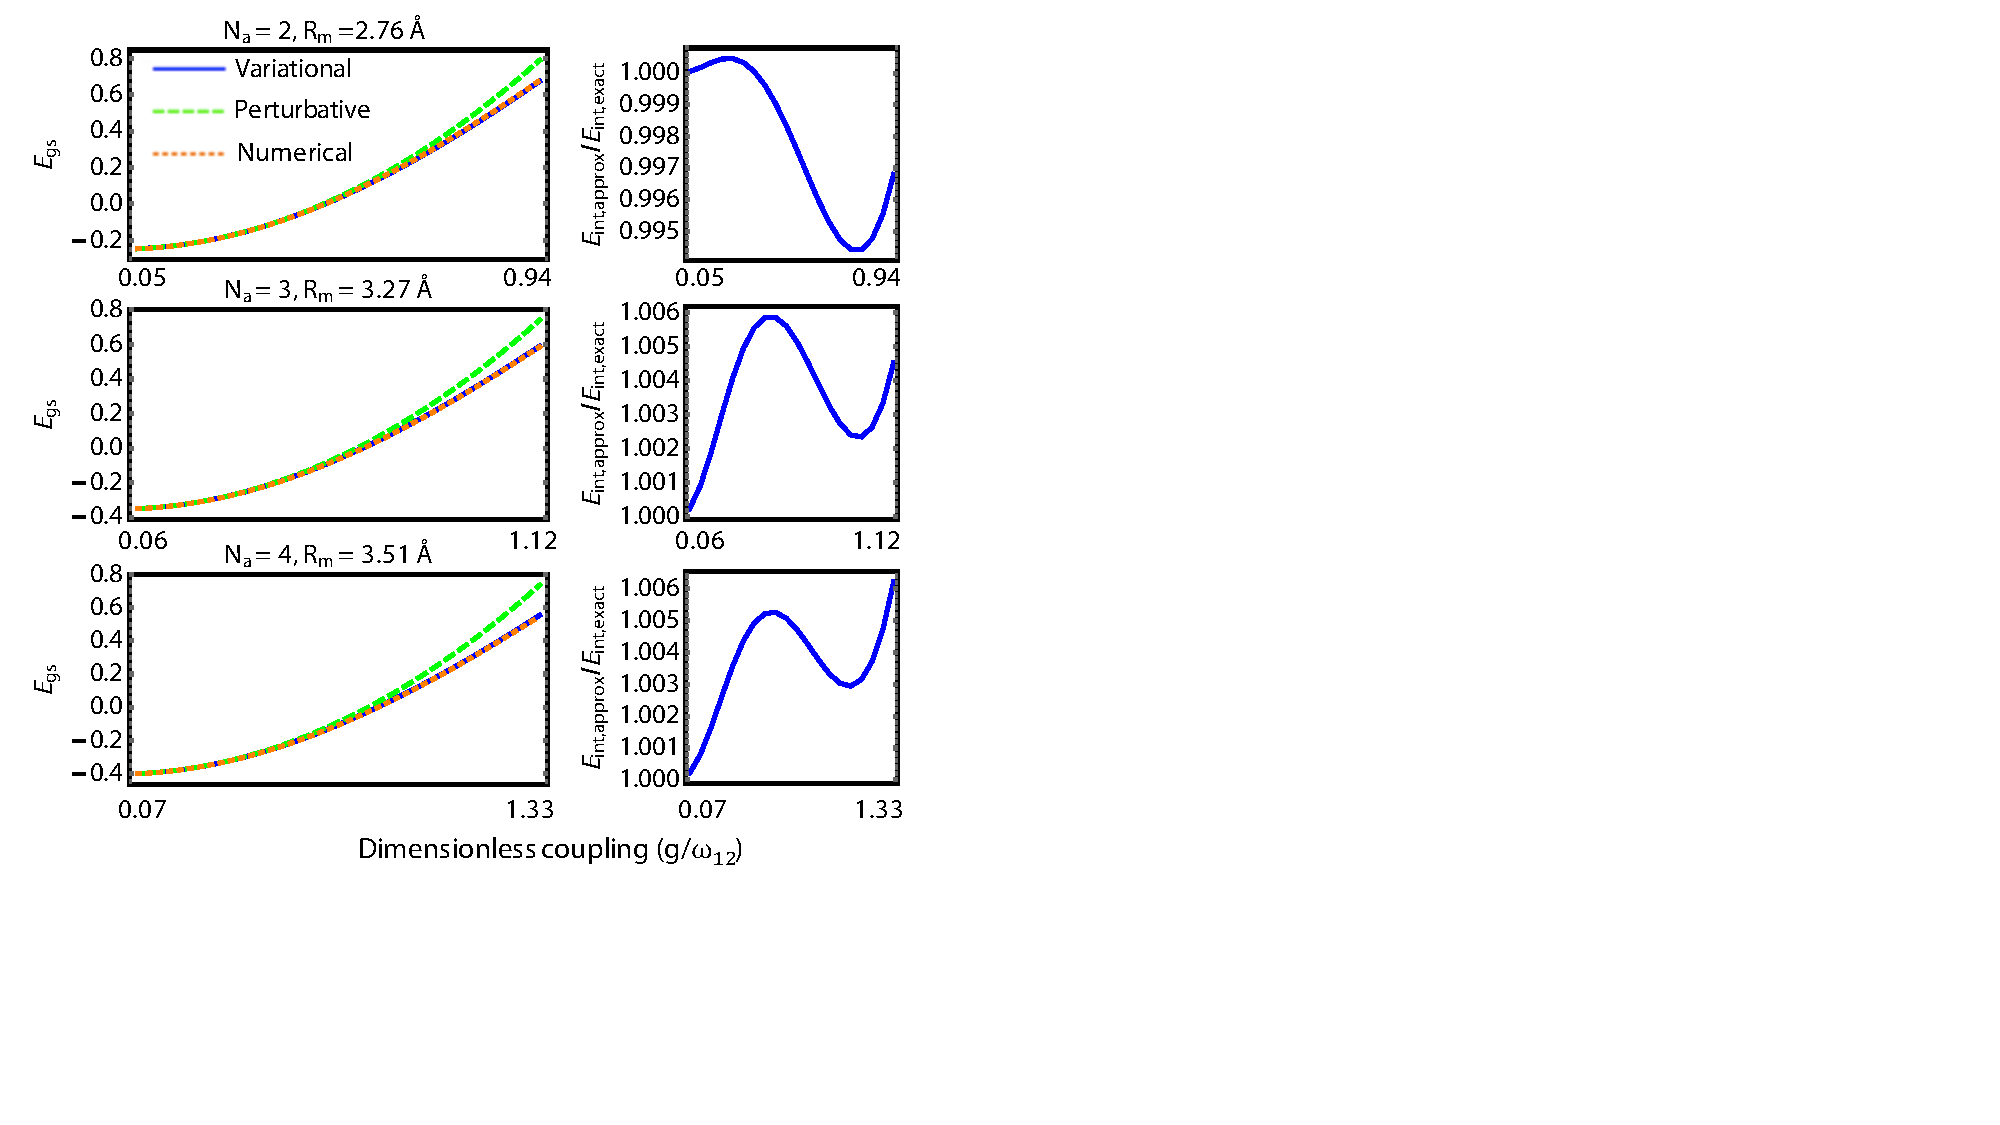
\includegraphics[width=8.4cm]{figure3new.pdf}
%\caption{\textbf{Variational theory of ground state energy: accuracy as a function of number of emitter levels.} (Left) Ground-state energy of the one-dimensional multi-mode Rabi model as a function of the dimensionless coupling for two (top), three (middle), and four (bottom) level emitter systems with momentum matrix elements chosen to saturate the Thomas-Reiche-Kuhn sum rule. (Right) Ratio of the energy calculated with the variational theory and with numerical diagonalization. These results show that our accuracy is robust to the number of levels in the system. }
%\label{fig:ansatz}
%\end{figure}

In what follows, we provide a proof-of-concept demonstration of the accuracy and content of the variational theory derived here. We consider the QED Hamiltonian corresponding to a single emitter placed at position $z=d$ in a one-dimensional cavity whose axis is along the $z$-direction. As the cavity is considered for simplicity to be one-dimensional, the electric field is oriented along a single direction, denoted $x$, while the magnetic field is oriented along a direction transverse to both the electric field and the cavity length, denoted $y$. Working under the long-wavelength (dipole) approximation, the Hamiltonian can then be written as:
\begin{equation}\label{eq:hamiltonian}
H = H_{\text{matter}}+\frac{\epsilon_0S}{2}\int dz~(E^2+c^2B^2)+\frac{q}{m}A(d)p + \frac{q^2}{2m}A^2(d),
\end{equation}
with the emitter charge now expressed as $q$, $E, B$, and $A$ being the electric field, magnetic field, and vector potential, and $S$ being a normalization area of the cavity in the $xy$ plane. The fields can be expressed as a mode expansion, where for a cavity of length $L$, the modes are given by $F_n(z) = \sqrt{\frac{2}{L}}\sin\left(\frac{n\pi z}{L} \right)$ and the corresponding mode frequencies are $\omega_n = \frac{n\pi c}{L}$. The matter Hamiltonian we take to be a multilevel system with $N_a$ levels. The matter system we describe can thus be mapped to an $N_a$ site system, which be considered as a simplified model of a molecule within a tight-binding description. Thus we parameterize the general family of matter Hamiltonians as:
\begin{equation}\label{eq:matter_hamiltonian}
H_{\text{matter}} = \sum\limits_{i=1}^{{N_a-1}} V_i|i\rangle\langle i|+t(|i\rangle\langle i+1|+|i+1\rangle\langle i|).
\end{equation}
The momentum operator, we write as 
\begin{equation}\label{eq:momentum_operator}
p = \frac{-i\hbar}{R}\sum\limits_{i=1}^{N_a-1} \left(|i\rangle\langle i+1|-|i+1\rangle\langle i| \right),
\end{equation}
where $R$ is a constant with units of length representing roughly the difference in positions between sites. This physical interpretation however is rough: it is also a function of the hopping elements $t$, because we choose $R$ in this work such that the Thomas-Reiche-Kuhn (TRK) sum rule is enforced: $\frac{2}{m}\sum\limits_{i=2}^{N_a}\frac{|p_{ig}|^2}{E_i - E_a} = 1$, where $p_{ig} = \langle i|p|g\rangle$ are momentum matrix elements between different matter states \cite{cohen1992}.  Since the sum rule is based on a full electronic real-space description, it does not rigorously apply to a discrete-level system. However, the matrix elements and energy levels of a few-level approximated Hamiltonian are derived from an underlying real-space Hamiltonian. Thus, a discrete system which has  $\frac{2}{m}\sum\limits_{i=2}^{N_a}\frac{|p_{ig}|^2}{E_i - E_a} > 1$ cannot exist physically. The TRK sum rule places a bound on how strong the effect of the $A\cdot p$ term can be. The net effect is that the value of $R$ we choose is on the order of $\sqrt{\frac{\hbar}{2mt}}$. These considerations also imply that when we plot observables as a function of some coupling parameter, for fixed $R$, we must vary a parameter which does not explicitly appear in the sum rule such as the charge or the number of emitters in the cavity.

The detailed derivations of the energies of states via the formalism introduced here are shown in the Supplementary Materials (SM). Here, we state the main results. Using a one-dimensional version of Eq. (\ref{eq:mhf-electron}) and (\ref{eq:mhf-photon}), we calculate the electron orbitals, photon orbitals, and photon frequencies in the absence of correlations. In the absence of correlations, we found for example that the energy of any matter state $a$ with no photonic quasiparticles is given by:
\begin{equation}
E_{a} = E^{0}_a + \frac{1}{2}\sum\limits_{n=1}^{\infty}(\hbar\omega_n - \hbar\omega_n^0),
\label{eq:casimir}
\end{equation}
where $E_a^0$ is the energy of the matter state in the absence of coupling, $\omega_n$ are found in our framework, $\omega_n^0 = \frac{n\pi c}{L}$. Imposing continuity of the modes and discontinuity of their derivatives at $z=d$, the modes found in our framework have their frequencies given by
\begin{equation}
\cot\left(\frac{\omega_n}{c}d \right)+\cot\left(\frac{\omega_n}{c}(L-d) \right) = -\frac{q^2}{m\epsilon_0\omega_nc}.
\label{eq:cot}
\end{equation}
The corresponding `interacting' field mode profiles are given by
\begin{align}\label{eq:field_mode}
N_n^{-1}F_n(z) =~ &\theta(z-d) \left(\frac{\sin\left(\frac{\omega_nL}{c}\right)\sin\left(\frac{\omega_nd}{c}\right)\cos\left(\frac{\omega_nz}{c}\right)}{\sin\left(\frac{\omega_n(L-d)}{c}\right)}\right) \nonumber \\ 
-&\theta (z-d) \left(\frac{\cos\left(\frac{\omega_nL}{c}\right)\sin\left(\frac{\omega_nd}{c}\right)\sin\left(\frac{\omega_nz}{c}\right)}{\sin\left(\frac{\omega_n(L-d)}{c}\right)}\right) \nonumber \\ 
+&\theta (d-z) \sin\left(\frac{\omega_n z}{c} \right),
\end{align}
with the normalization constant
\begin{equation}\label{eq:mode_normalization}
N_n = 2\sqrt{\frac{1}{\frac{c}{\omega_n}\left(\frac{\omega_nL}{c}-\sin\left(\frac{\omega_nL}{c}\right) \right)\left(1+\frac{\sin^2\left(\frac{\omega_nd}{c}\right)}{\sin^2\left(\frac{\omega_n(L-d)}{c}\right)} \right)}}.
\end{equation}
The result of Eq. (\ref{eq:casimir})  says that in the absence of correlations, the energy of the system is the Casimir energy of the system. In particular, it has long been known that when two conducting plates are placed near each other, there is a Casimir energy associated with the fact that the zero-point energy of the nearby plates is different than the zero-point energy of plates infinitely apart. This is because the electromagnetic mode structure of two nearby plates is different from that of two infinitely separated plates. This Casimir energy is simply the difference between the interacting and non-interacting zero-point energies \cite{casimir1948attraction,lifshitz1956theory}. This logic can be applied to any arrangement of macroscopic polarizable objects. What is notable about the result of Eq. (\ref{eq:casimir}) is it implies that the same logic about zero-point energy differences can be applied to find the interaction energy case of a \textit{single atom} placed near a cavity, even though a single emitter is very far from the limit of a macroscopic polarizable object. 
\begin{figure}[t]
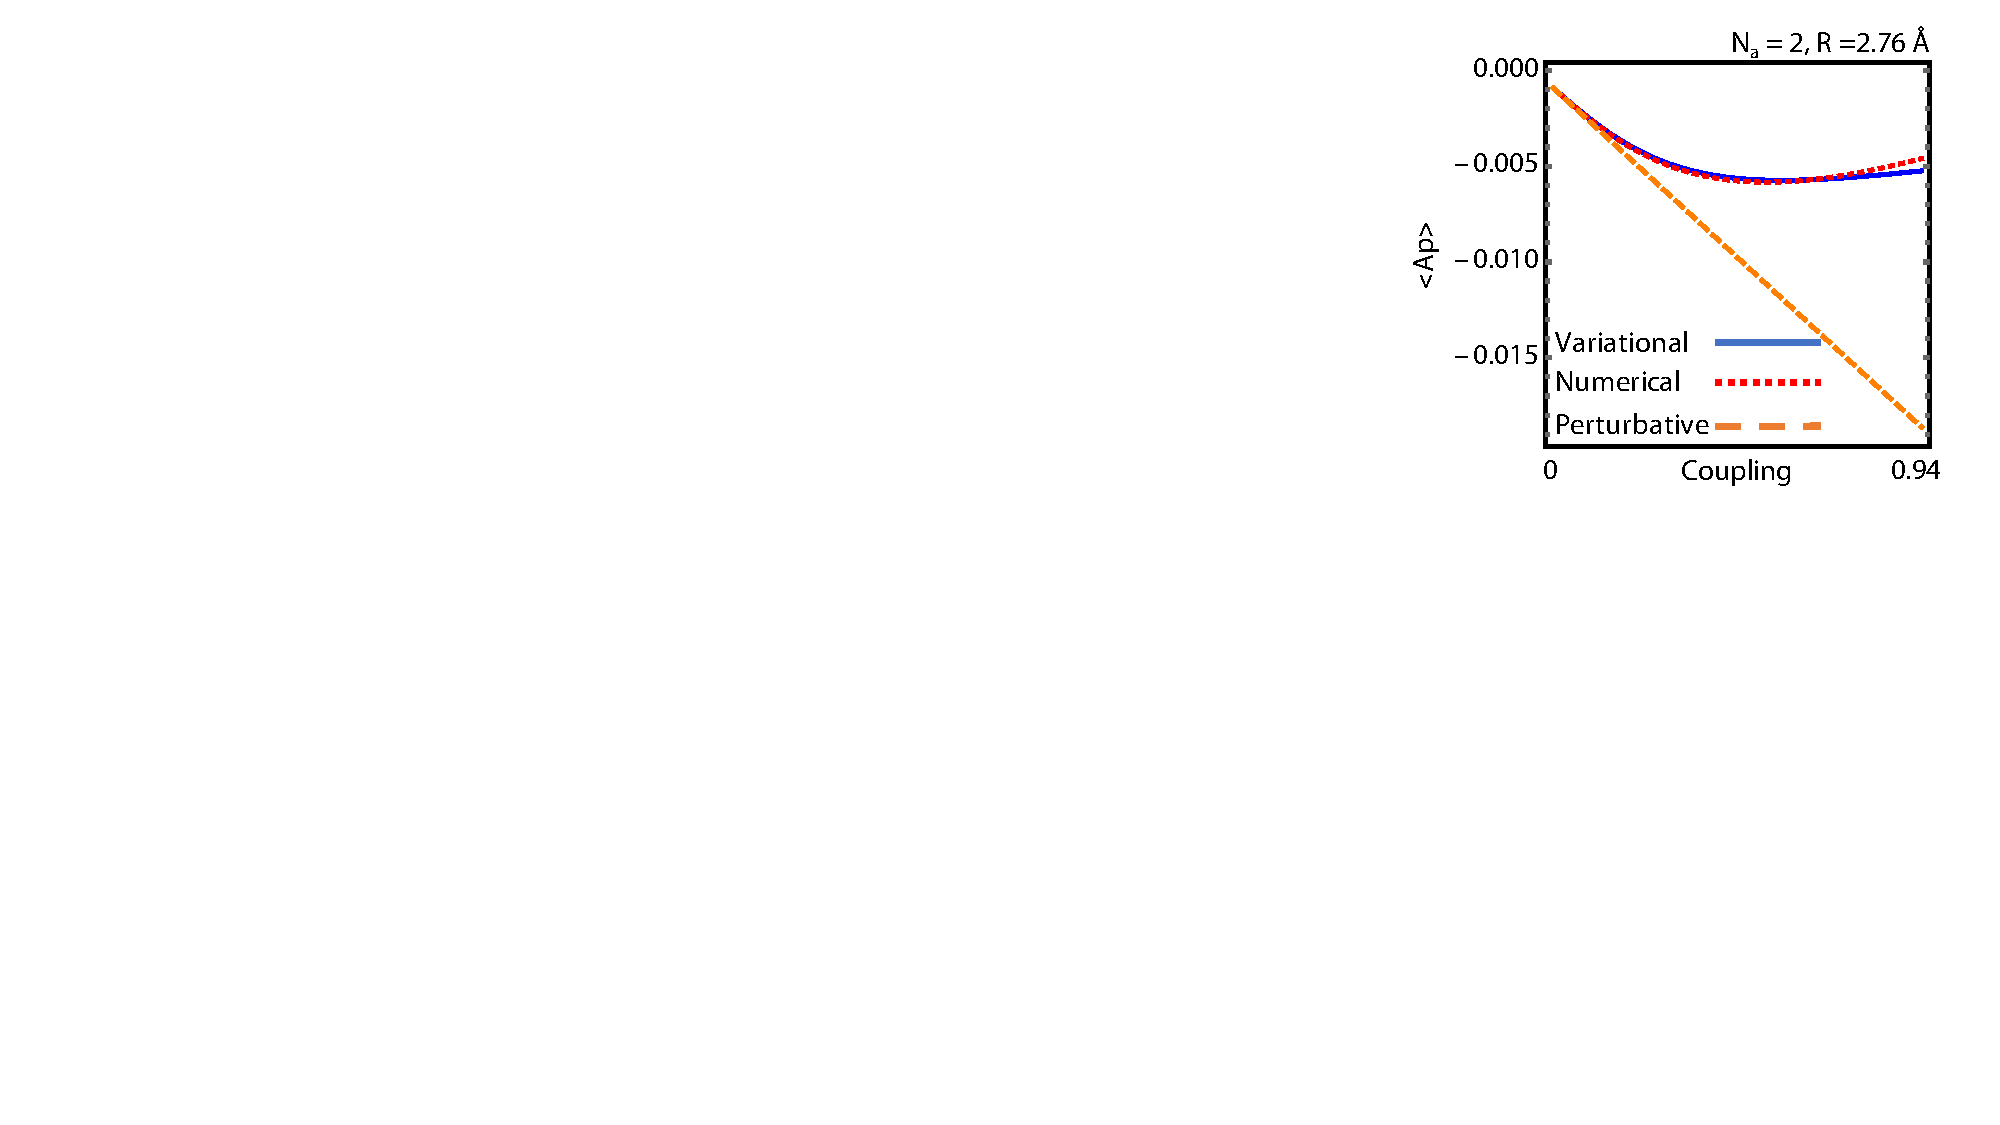
\includegraphics[width=6cm]{figure3revision.pdf}
\caption{\textcolor{blue}{\textbf{Expectation value of the correlated observable $\langle A\cdot p \rangle $ as a function of coupling.} Parameters are identical to those of the top panel of Fig. 2a, and show that despite correlations being treated perturbatively, they are in excellent agreement with exact diagonalization, while in poor qualitative and quantitative agreement with perturbation theory in the bare photonic modes.}}
\label{fig:correlated}
\end{figure}
In the presence of correlations  we must add to the energy a contribution of the form of Eq. (\ref{eq:e-shift}), specialized to the case of an emitter in a one-dimensional cavity. The interaction energy, given by Eqs. (\ref{eq:e-shift}) and (\ref{eq:casimir}) is semi-analytical once the bare emitter states are known, as it is fully specified by Eqs. (\ref{eq:cot}-\ref{eq:mode_normalization}) once the transcendental equation of Eq. (\ref{eq:cot}) is solved. We also apply the correlation correction to excited states as well, by using the second-order perturbation theory formula for the energy shift of excited states due to the $A \cdot p$ term, using the same electron and photon orbitals and frequencies as derived in Eqs. (\ref{eq:mhf-electron}) and (\ref{eq:mhf-photon}). In Fig. ~\ref{fig:results}(a), we show the result of this procedure when applied to calculate ground- and excited- state energies for two-, three-, and four-level systems coupled to a one-dimensional cavity. The relevant parameters for Fig. 2(a) are listed in the SM. \textcolor{blue}{For the largest couplings considered here, the magnitude of the energy shift associated with the $A \cdot p$ term predicted from perturbation theory is larger than the energy separation between bare emitter levels, signaling the ultrastrong coupling regime.} 

In all cases, the agreement between our variational approach and numerical diagonalization is excellent, suggesting that our variational method is sufficiently flexible to capture ground states and excited states both with and without photonic excitations. The accuracy as a function of number of levels suggests that the breakdown of gauge invariance associated with few-level systems is not crucial to the good agreement between variational and numerical results \cite{bernardis2018breakdown}. This is to be contrasted with perturbation theory in the bare matter and photon states, which can both strongly over- and underestimate the energies. The most interesting case of disagreement arises in the case of the two-level system (top panel). For the two-level system considered here, the variational result agrees very well with numerical diagonalization, while perturbation theory predicts an energy which evolves with coupling in the wrong direction and is off from the true energy by over 100\%.

Importantly, the reason perturbation theory fails for first excited state, much more so than for the ground state, is that the first bare cavity mode is nearly resonant with the transition between ground and excited emitter states, leading to a very large negative contribution from the $A\cdot p$ of nearly $2$ eV, which is far larger than the spacing of the bare emitter levels. On the other hand, the variational estimate from our formalism finds no such large negative energy shift, and leads to an energy gap between the first two levels which is similar to the bare gap, and in agreement with numerical diagonalization. The reason for this behavior is that the effect of the plasma term in Eq. (\ref{eq:mhf-photon}) is to blue-shift all of the photon frequencies. In particular, for the largest coupling considered in Figure~\ref{fig:results}, we find that the lowest photon frequency is shifted to 0.99 eV, and then becomes far off-resonance from the bare emitter transition. The plasma term, as shown in Fig.~\ref{fig:results}b, also strongly reduces the coupling between light and matter by a different mechanism in which the field modes obtained from Equation (\ref{eq:mhf-photon}) are screened out of the emitter, thus self-consistently reducing the strength of the coupling between matter and field and the magnitude of the correlation term, as per Equation (\ref{eq:e-shift}). This is a so-called light-matter decoupling effect, which was proposed in Ref. ~\cite{liberato2014}. \textcolor{blue}{In Ref. ~\cite{liberato2014}, on the basis of photodetection probabilities for exactly-obtained excited polaritonic eigenstates in a Hopfield model, deLiberato obtained "effective field mode profiles" with a strong dip in the location of the emitter, in qualitative agreement with what we report here.}

\textcolor{blue}{This mechanism is also reflected in Fig. ~\ref{fig:correlated}, where we calculate a correlated ground state observable such as $\langle Ap \rangle$, which is a measure of entanglement between the ground state and excitations of the photon and matter (details shown in Supplemental Materials). Such observables may play a role in correlated spectroscopies, as proposed in Ref. ~\cite{flick2017}. We show predictions of the value of this observable based on the variational method, numerical diagonalization, and perturbation theory in the bare emitter and photon states. As can be seen, perturbation theory overestimates the magnitude of the energy shift, while both numerical and variational methods capture a saturation and then decrease of this expectation value, showing an apparent de-correlation between light and matter in the deep-strong coupling regime. The results of Fig. ~\ref{fig:results} and \ref{fig:correlated}  demonstrate not only the accuracy of our ansatz, but provides insight into the mechanisms by which light-matter coupling saturates in the nonperturbative QED regime. The results of Fig. ~\ref{fig:results} and \ref{fig:correlated} also show that despite correlations being treated perturbatively, it remains possible for correlated observables (and energies) to be predicted with high accuracy.}

Our results also demonstrate a non-perturbative theory of the Lamb shift and consequently Casimir-Polder forces. In particular, it is long known that energy levels of emitters can shift as a result of virtual photon emission and re-absorption. These energy shifts, called Lamb shifts, depend on the particular position of the emitter in the photonic structure it is embedded in. These shifts not only lead to changes in the transition frequencies of the emitter, but the position dependence of these energy shifts also implies forces on the emitter, often called Casimir-Polder forces. Such forces are calculated by applying second-order perturbation theory in the form of Eq. (\ref{eq:e-shift}) using \textit{bare} atomic and photonic properties \cite{scheel2009macroscopic}. Our calculation of the Lamb shifts via Eq. (\ref{eq:e-shift}) says that the shifts result from virtual emission and re-absorption of the photonic quasiparticles (the \textit{interacting} modes), governed by (Eqs. (\ref{eq:cot}-\ref{eq:mode_normalization})), which are dependent on properties of the matter. As these interacting photon modes differ greatly from the bare modes and frequencies in the non-perturbative regime, Eq. (\ref{eq:e-shift}) using interacting modes provides a compact, and conceptually simple extension of the theory of Lamb shifts and Casimir-Polder forces to the non-perturbative regime.

With the advent of ultra-strong coupling and deep-strong coupling in QED systems, the theory posed here, when applied to more complex systems, could form the basis for understanding Lamb and Casimir phenomena in the ultra-strong coupling regime. Additionally, the results developed here could be applied to capture spontaneous emission in the non-perturbative regime. Finally, one could use the non-perturbative real-space knowledge of how matter affects photons in order to design a photonic mode atom-by-atom.

%In Figure 3, we consider the ground state of the QED Hamiltonian, calculated through the procedure above, but now extended to three and four level systems. In all cases, the parameter $R$ is chosen to saturate the TRK sum rule. We find that the accuracy of our approach is not compromised by having additional energy levels in the Hamiltonian, indicating the potential of our approach.

%Finally, we note that Eq. (8), which incorporates correlations, can also be employed self-consistently, by adding it to the Lagrange function of Eq. (5), and minimizing the result with respect to electronic and photonic properties. The set of equations that arise are \Jadd{(Nick, should we remove the argument in F(\mathbf{x}) in the following equation?)}:
%%\vspace{-1.5cm}
%\begin{widetext}
%\begin{align}
%&\left(\frac{\mathbf{p}^2}{2m}+v_{\mathrm{ext}}(\mathbf{x}) \right)\psi_i(\mathbf{x}) +  \sum\limits_{j=1}^N \int d^3x' ~ V(\mathbf{x}-\mathbf{x}')\left(\psi^*_j(\mathbf{x}')\psi_j(\mathbf{x}')\psi_i(\mathbf{x}) - \psi_j(\mathbf{x}')\psi_j(\mathbf{x})\psi_i(\mathbf{x}')  \right) \nonumber \\ &+ \frac{\hbar e^2}{4m\epsilon_0}\sum_n \frac{1}{\omega_n}|\mathbf{F}_n|^2\psi_i(\mathbf{x}) + \frac{e^2\hbar^2}{8m^2\epsilon_0}\sum\limits_{n=N_{\sigma}+1}^{\infty}\sum\limits_{q=1}^{N_p} \frac{\int d^3y~\mathbf{F}^*_q(\mathbf{y})\cdot\mathbf{j}_{ni}(\mathbf{y})}{\omega_q(\omega_{in}-\lambda_q)}\left( \mathbf{F}_q(\mathbf{x})\cdot\nabla\psi_n(\mathbf{x}) + \nabla\cdot(\mathbf{F}_q(\mathbf{x})\psi_n(\mathbf{x}))\right)  = E_i\psi_i(\mathbf{x}).
%\end{align}
%\end{widetext}
%
%\begin{widetext}
%\begin{equation}
%\left( \nabla\times\nabla\times - \left(1-\frac{\omega_p^2}{\omega_q^2} \right)\right)\mathbf{F}_q = -\frac{e^2\hbar}{2m^2\epsilon_0c^2}\sum\limits_{n=N_{\sigma}+1}^{\infty}\sum\limits_{m=1}^{N_{\sigma}} \frac{\int d^3y~\mathbf{F}_q(\mathbf{y})\cdot\mathbf{j}_{mn}(\mathbf{y})}{\omega_{mn}-\omega_{q}}\mathbf{j}_{nm}.
%\end{equation}
%\end{widetext}
%Eqs. (13) and (14) are quite general, providing real-space information about the electronic and photonic properties of the QED ground state for a many-electron system in a many-mode system in three dimensions. 


%In summary, we have developed a variational approximation to the ground state of quantum electrodynamical problems and have benchmarked it against the multi-mode and multi-level Rabi model, which has no analytical solutions, and whose accurate numerical diagonalization requires a very high-dimensional Hilbert space. Despite our ansatz being centered on the assumption of weak correlations, with correlations from the $Ap$ term being treated perturbatively, we find that our approximation does very well in predicting the ground state energy, even when the strength of the correlations saturates the TRK sum rule.  

%In what follows, we add this energy correction $\delta E$ to the expectation value of the energy in the ground state, with the orbitals and eigenvalues as variational parameters. As a result, the orbitals and eigenvalues obtained will be different from Eq. (11) and (14), and this difference will be small in the limit of weak correlations. Strictly speaking, this approach is only justified for weak correlations, but can be applied to systems with strong-correlations as is often done with self-consistent methods. Minimizing with respect to the orbitals, photon modes, and photon frequencies, immediately yields:
%\begin{widetext}
%\begin{align}
%&\left(\frac{\mathbf{p}^2}{2m}+v_{\mathrm{ext}}(\mathbf{x}) \right)\psi_i(\mathbf{x}) +  \sum\limits_{j=1}^N \int d^3x' ~ V(\mathbf{x}-\mathbf{x}')\left(\psi^*_j(\mathbf{x}')\psi_j(\mathbf{x}')\psi_i(\mathbf{x}) - \psi_j(\mathbf{x}')\psi_j(\mathbf{x})\psi_i(\mathbf{x}')  \right) \nonumber \\ &+ \frac{\hbar e^2}{4m\epsilon_0}\sum_n \frac{1}{\omega_n}|\mathbf{F}_n|^2\psi_i(\mathbf{x}) + \frac{e^2\hbar^2}{8m^2\epsilon_0}\sum\limits_{n=N_{\sigma}+1}^{\infty}\sum\limits_{q=1}^{N_p} \frac{\int d^3y~\mathbf{F}^*_q(\mathbf{y})\cdot\mathbf{j}_{ni}(\mathbf{y})}{\omega_q(\omega_{in}-\lambda_q)}\left( \mathbf{F}_q(\mathbf{x})\cdot\nabla\psi_n(\mathbf{x}) + \nabla\cdot(\mathbf{F}_q(\mathbf{x})\psi_n(\mathbf{x}))\right)  = E_i\psi_i(\mathbf{x}).
%\end{align}
%\end{widetext}
%
%\begin{widetext}
%\begin{equation}
%\left( \nabla\times\nabla\times - \left(1-\frac{\omega_p^2}{\omega_q^2} \right)\right)\mathbf{F}_q = -\frac{e^2\hbar}{2m^2\epsilon_0c^2}\sum\limits_{n=N_{\sigma}+1}^{\infty}\sum\limits_{m=1}^{N_{\sigma}} \frac{\int d^3y~\mathbf{F}_q(\mathbf{y})\cdot\mathbf{j}_{mn}(\mathbf{y})}{\omega_{mn}-\omega_{q}}\mathbf{j}_{nm}.
%\end{equation}
%\end{widetext}
%These two equations are highly general, providing real-space information about the electronic and photonic properties of the QED ground state for a many-electron system in a many-mode system in three dimensions. Commensurately, these equations are complicated, and to understand them, we now consider a simple case of them.  




%\section{Summary and Outlook}
%In summary, we have developed a variational approximation to the ground state of quantum electrodynamical problems and have benchmarked it against the multi-mode and multi-level Rabi model, which has no analytical solutions, and whose accurate numerical diagonalization requires a very high-dimensional Hilbert space. Despite our ansatz being centered on the assumption of weak correlations, with correlations from the $Ap$ term being treated perturbatively, we find that our approximation does very well in predicting the ground state energy, even when the strength of the correlations saturates the TRK sum rule. 

%From a more fundamental perspective, the ansatz studied in this work is interesting because they give a rigorous meaning to the notion of correlation energy in quantum electrodynamics which is parallel to correlation energy in electronic structure theory. In particular, in the context of electronic structure, the correlation energy is the difference between the true ground state energy and that computed by Hartree-Fock, which is an independent electron ansatz. Similarly, our ansatz here is an independent electron-independent photon ansatz whose structure is parallel to the Hartree-Fock ansatz. 

%Another fundamentally interesting aspect of our ansatz is that unlike current formulations of quantum-electrodynamical density functional theory, it considers the real-space properties of photon modes as they are affected by matter. With the advent of ultra-strong coupling and deep-strong coupling being realizable in quantum electrodynamical systems, one may use this real-space knowledge of how matter affect photons to design a photonic mode atom-by-atom.

%\section{Acknowledgements}
%We thank Prof. Joel Yuen-Zhou (University of California San Diego), Prof. Ido Kaminer (Technion Israel Institute of Technology), Prof. Marin Solja\v{c}i\'{c} (Massachusetts Institute of Technology) and Prof. John D. Joannopoulos (Massachusetts Institute of Technology), for useful discussions. N. R. recognizes the support of the DOE Computational Science Graduate Fellowship (CSGF) fellowship no.  DE-FG02-97ER25308. J. F. acknowledges financial support from the Deutsche Forschungsgemeinschaft (DFG Forschungsstipendium FL 997/1-1). This work was supported by the DOE Photonics at Thermodynamic Limits Energy Frontier Research Center under grant no. DE-SC0019140.



\bibliographystyle{apsrev4-1}
\bibliography{references}

\end{document}
